\subsection{Quantitative and Qualitative Results}
\label{sec:results}

% Table 1 — paste full numbers from the manuscript; do not invent values
% Table 1 — data from latex/MipNeRF360数据集/formatting-instructions-latex.tex (unchanged numbers)
\begin{table}[ht!]
\centering
\caption{\label{tab:mip360} Performance comparisons of sparse-view synthesis on Mip-NeRF 360 (4/6/9 views). LPIPS$^{*}$ denotes LPIPS $\times 10^{2}$.}
\setlength{\tabcolsep}{2.8mm}
\renewcommand{\arraystretch}{1.08}
\adjustbox{width=1\linewidth}{%
\begin{tabular}{c l | ccc | ccc | ccc}
\toprule
\multirow{2}{*}{}
  & \multirow{2}{*}{Methods}
  & \multicolumn{3}{c|}{Mip-NeRF 360 (4-view)}
  & \multicolumn{3}{c|}{Mip-NeRF 360 (6-view)}
  & \multicolumn{3}{c}{Mip-NeRF 360 (9-view)} \\
&
  & LPIPS$^{*}$$\downarrow$ & PSNR$\uparrow$ & SSIM$\uparrow$
  & LPIPS$^{*}$$\downarrow$ & PSNR$\uparrow$ & SSIM$\uparrow$
  & LPIPS$^{*}$$\downarrow$ & PSNR$\uparrow$ & SSIM$\uparrow$ \\
\midrule
\sidelabel{2}{NeRF-based}
  & RegNeRF
      & 19.88 & 12.59 & 0.841
      & 20.72 & 13.41 & 0.847
      & 19.70 & 13.68 & 0.852 \\
  & SparseNeRF
      & 17.76 & 12.83 & 0.845
      & 19.74 & 13.42 & 0.861
      & 21.56 & 14.36 & 0.873 \\
\addlinespace[4pt]
\sidelabel{5}{3DGS-based}
  & 3DGS
      &10.80 & 20.31 & 0.899
      &8.38 & 22.12 & 0.913
      &6.42 & 24.29 & 0.930 \\
  & CoR-GS
      &11.76 & 20.45 & 0.856
      &9.28 & 22.57 & 0.901
      &7.04 & 24.73 & 0.926 \\
  & DropGaussian
      &11.57 & 21.76 & 0.837
      &8.61 & 22.98 & 0.895
      &8.02 & 24.10 & 0.915 \\
  & D$^2$GS
      &\cellcolor{color_blue}2.58 &\cellcolor{blue!8}22.35 &\cellcolor{blue!8}0.923
      &\cellcolor{color_blue}2.34 &\cellcolor{blue!8}24.74 &\cellcolor{blue!8}0.937
      &\cellcolor{color_blue}2.11 &\cellcolor{blue!8}27.13 &\cellcolor{blue!8}0.941 \\
  & SynGS (Ours)
      &\cellcolor{blue!8}3.89 &\cellcolor{color_blue}25.91 &\cellcolor{color_blue}0.948
      &\cellcolor{blue!8}3.43 &\cellcolor{color_blue}27.93 &\cellcolor{color_blue}0.953
      &\cellcolor{blue!8}3.02 &\cellcolor{color_blue}29.21 &\cellcolor{color_blue}0.961 \\
\bottomrule
\end{tabular}%
}
\end{table}

% Table 2 — data from latex/FFLL数据集/formatting-instructions-latex.tex (unchanged numbers)
\begin{table}[ht!]
\centering
\caption{\label{tab:llff} Performance comparisons of sparse-view synthesis on the LLFF 360 dataset (4/6/9 views). LPIPS$^{*}$ denotes LPIPS $\times 10^{2}$.}
\setlength{\tabcolsep}{2.8mm}
\renewcommand{\arraystretch}{1}
\adjustbox{width=1\linewidth}{%
\begin{tabular}{c c | ccc | ccc | ccc}
\toprule
\multirow{2}{*}{}
  & \multirow{2}{*}{\centering Methods}
  & \multicolumn{3}{c|}{LLFF 360 (4-view)}
  & \multicolumn{3}{c|}{LLFF 360 (6-view)}
  & \multicolumn{3}{c}{LLFF 360 (9-view)} \\
&
  & LPIPS$^{*}$$\downarrow$ & PSNR$\uparrow$ & SSIM$\uparrow$
  & LPIPS$^{*}$$\downarrow$ & PSNR$\uparrow$ & SSIM$\uparrow$
  & LPIPS$^{*}$$\downarrow$ & PSNR$\uparrow$ & SSIM$\uparrow$ \\
\toprule
\multirow{4}{*}{\rotatebox{90}{\scriptsize NeRF-based}}
  & RegNeRF
      & 29.65 & 18.55 & 0.587
      & 22.61 & 19.08 & 0.760
      & 18.39 & 22.86 & 0.820 \\
  & FreeNeRF
      & 30.85 & 19.09 & 0.624
      & 23.06 & 19.81 & 0.763
      & 17.94 & 23.08 & 0.823 \\
\multirow{8}{*}{\rotatebox{90}{\scriptsize 3DGS-based}}
  & 3DGS
      &22.93 & 19.32 & 0.649
      &13.45 & 23.80 & 0.814
      &9.68 & 25.44 & 0.860 \\
  & CoR-GS
      &19.66 & 20.45 & 0.696
      &\cellcolor{color_blue}12.53 & 23.87 & 0.840
      &\cellcolor{color_blue}8.94 & 26.70 &\cellcolor{color_blue}0.874 \\
  & DropGaussian
      &21.93 & 19.80 & 0.621
      &13.79 & 23.41 & 0.803
      &9.40 & 25.87 & 0.868 \\
  & D$^2$GS
      &\cellcolor{blue!8}17.98 &\cellcolor{blue!8}22.35 &\cellcolor{blue!8}0.746
      &13.85 &\cellcolor{blue!8}23.91 &\cellcolor{blue!8}0.846
      &8.91 &\cellcolor{color_blue}26.80 &\cellcolor{blue!8}0.871 \\
  & SynGS (Ours)
      &\cellcolor{color_blue}16.92 &\cellcolor{color_blue}23.92 &\cellcolor{color_blue}0.762
      &\cellcolor{blue!8}12.54 &\cellcolor{color_blue}25.17 &\cellcolor{color_blue}0.848
      &\cellcolor{blue!8}8.96 &\cellcolor{blue!8}26.71 &\cellcolor{blue!8}0.871 \\
\toprule
\end{tabular}%
}
\end{table}


\textbf{Mip-NeRF 360 and LLFF.}
Table~\ref{tab:mip360} reports the results on Mip-NeRF 360 under the 4-, 6-, and 9-view settings. SynGS achieves the highest PSNR and SSIM in all three settings, with the largest PSNR advantage in the 4-view case: 25.91~dB, 3.56~dB above D$^2$GS~\cite{Song26_D2GS}. For LPIPS, D$^2$GS obtains lower values across the three settings. Table~\ref{tab:llff} shows a similar trend. With four views, SynGS achieves the best PSNR, SSIM, and LPIPS; under six views it obtains the highest PSNR and SSIM with LPIPS close to the best result. At nine views, D$^2$GS~\cite{Song26_D2GS} gives slightly higher PSNR and lower LPIPS, while CoR-GS~\cite{Zhang24_CoRGS} achieves slightly higher SSIM. The clearest advantage appears in the 4- and 6-view settings.

\textbf{Qualitative Results.}
Figure~\ref{fig:qualitative} shows the 4-view comparison on Mip-NeRF 360. SynGS produces fewer floating artifacts and more complete object boundaries, and preserves finer structures where baselines show broken contours or missing details.

\begin{figure}[!htbp]
\centering
\setlength{\tabcolsep}{1.2pt}
\renewcommand{\arraystretch}{0.2}
\scriptsize
\begin{tabular}{@{}cccccccc@{}}
RegNeRF & SparseNeRF & 3DGS & CoR-GS & DropGaussian & D$^2$GS & SynGS (Ours) & GT \\
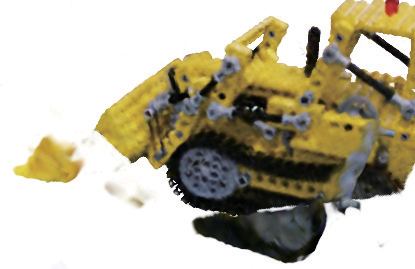
\includegraphics[width=0.118\textwidth]{figures/qualitative/s1_regnerf} &
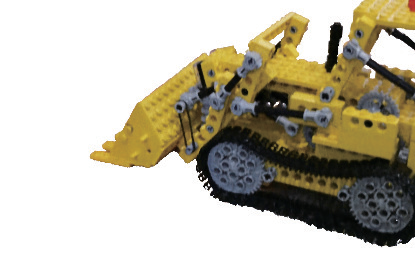
\includegraphics[width=0.118\textwidth]{figures/qualitative/s1_sparsenerf} &
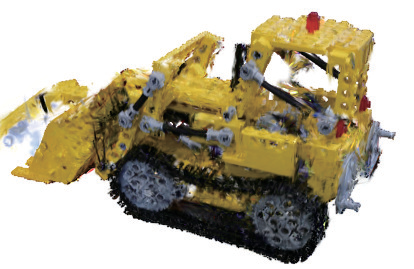
\includegraphics[width=0.118\textwidth]{figures/qualitative/s1_3dgs} &
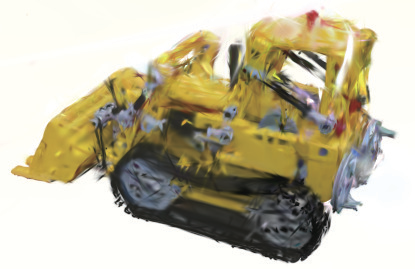
\includegraphics[width=0.118\textwidth]{figures/qualitative/s1_corgs} &
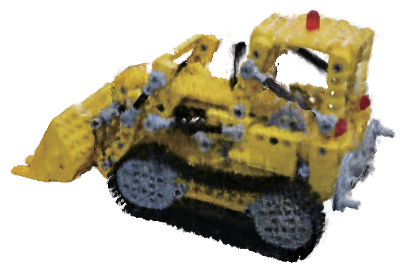
\includegraphics[width=0.118\textwidth]{figures/qualitative/s1_dropgaussian} &
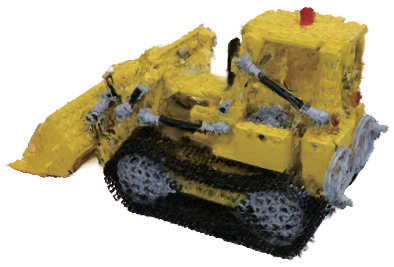
\includegraphics[width=0.118\textwidth]{figures/qualitative/s1_d2gs} &
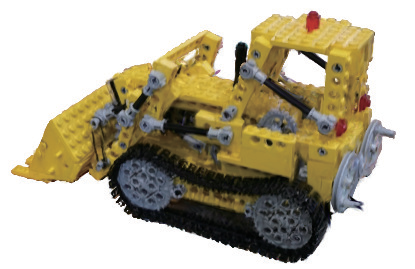
\includegraphics[width=0.118\textwidth]{figures/qualitative/s1_ours} &
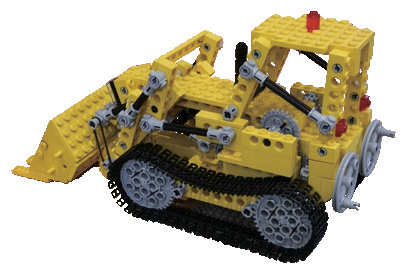
\includegraphics[width=0.118\textwidth]{figures/qualitative/s1_gt} \\[1pt]
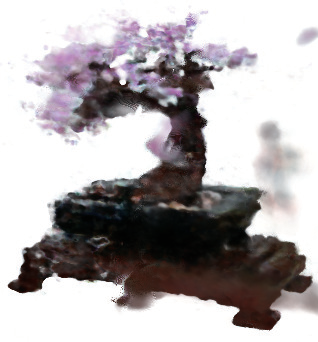
\includegraphics[width=0.118\textwidth]{figures/qualitative/s2_regnerf} &
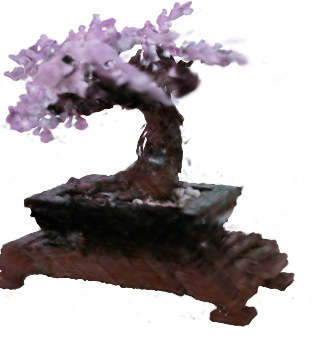
\includegraphics[width=0.118\textwidth]{figures/qualitative/s2_sparsenerf} &
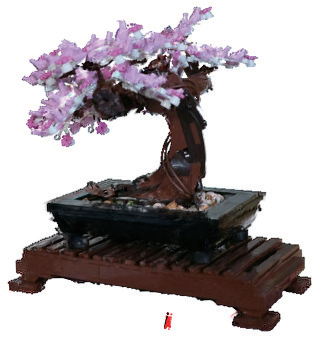
\includegraphics[width=0.118\textwidth]{figures/qualitative/s2_3dgs} &
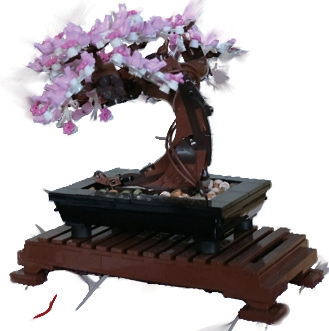
\includegraphics[width=0.118\textwidth]{figures/qualitative/s2_corgs} &
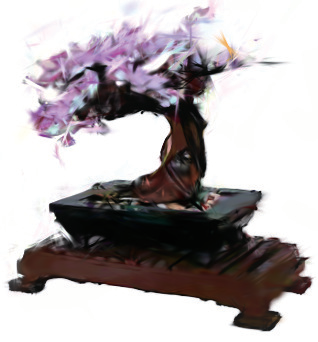
\includegraphics[width=0.118\textwidth]{figures/qualitative/s2_dropgaussian} &
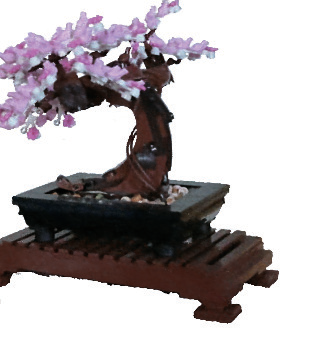
\includegraphics[width=0.118\textwidth]{figures/qualitative/s2_d2gs} &
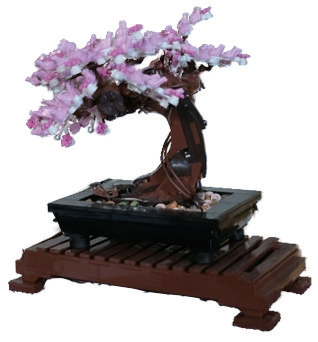
\includegraphics[width=0.118\textwidth]{figures/qualitative/s2_ours} &
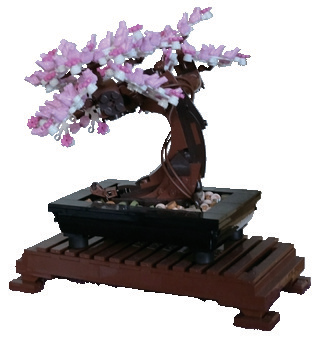
\includegraphics[width=0.118\textwidth]{figures/qualitative/s2_gt} \\[1pt]
\makebox[0.118\textwidth]{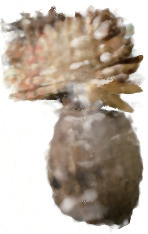
\includegraphics[height=0.127\textwidth]{figures/qualitative/s3_regnerf}} &
\makebox[0.118\textwidth]{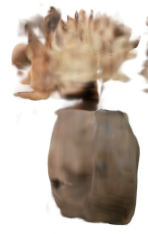
\includegraphics[height=0.127\textwidth]{figures/qualitative/s3_sparsenerf}} &
\makebox[0.118\textwidth]{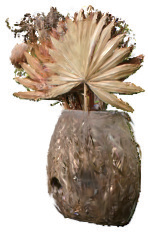
\includegraphics[height=0.127\textwidth]{figures/qualitative/s3_3dgs}} &
\makebox[0.118\textwidth]{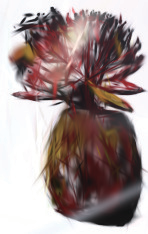
\includegraphics[height=0.127\textwidth]{figures/qualitative/s3_corgs}} &
\makebox[0.118\textwidth]{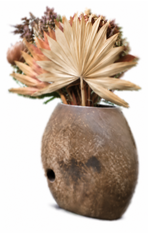
\includegraphics[height=0.127\textwidth]{figures/qualitative/s3_dropgaussian}} &
\makebox[0.118\textwidth]{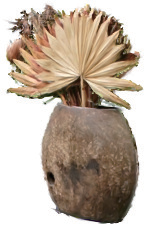
\includegraphics[height=0.127\textwidth]{figures/qualitative/s3_d2gs}} &
\makebox[0.118\textwidth]{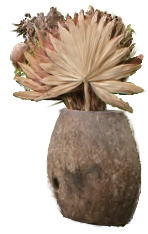
\includegraphics[height=0.127\textwidth]{figures/qualitative/s3_ours}} &
\makebox[0.118\textwidth]{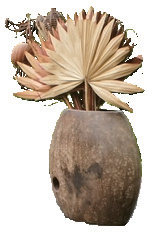
\includegraphics[height=0.127\textwidth]{figures/qualitative/s3_gt}}
\end{tabular}
\caption{\label{fig:qualitative} Qualitative comparison under the 4-view sparse-input setting on Mip-NeRF 360. SynGS produces fewer floating artifacts and more complete structural boundaries than the compared methods.}
\end{figure}
